\documentclass[a4paper, 11pt]{article}

\usepackage[left=1.5cm, right=1.5cm, top=2cm, bottom=2cm]{geometry}

\usepackage[utf8]{inputenc} 
\usepackage[T1]{fontenc}      
\usepackage[french,english]{babel}  
\usepackage{lmodern}

\usepackage{amsmath, mathtools}
\usepackage{amssymb}
\usepackage{amsthm}
\usepackage{empheq}

\usepackage{graphicx}
\usepackage{subfig}

\usepackage{listings}
\usepackage{color} %red, green, blue, yellow, cyan, magenta, black, white
\definecolor{mygreen}{RGB}{28,172,0} % color values Red, Green, Blue
\definecolor{mylilas}{RGB}{170,55,241}


\lstset{language=Matlab,%
    %basicstyle=\color{red},
    breaklines=true,%
    morekeywords={matlab2tikz},
    keywordstyle=\color{blue},%
    morekeywords=[2]{1}, keywordstyle=[2]{\color{black}},
    identifierstyle=\color{black},%
    stringstyle=\color{mylilas},
    commentstyle=\color{mygreen},%
    showstringspaces=false,%without this there will be a symbol in the places where there is a space
    numbers=left,%
    numberstyle={\tiny \color{black}},% size of the numbers
    numbersep=9pt, % this defines how far the numbers are from the text
    emph=[1]{for,end,break},emphstyle=[1]\color{red}, %some words to emphasise
    %emph=[2]{word1,word2}, emphstyle=[2]{style},    
}

\begin{document}
\title{Rendu TP1 Image sous-pixellique}
\author{Yoann Pradat}
\maketitle

\paragraph{Exercice 1}

%%%%%%%%%%%%
% Question 1
%%%%%%%%%%%%

1) On définit d'abord une fonction permettant de calculer la tâche de diffraction d'une source ponctuelle à travers une
ouverture circulaire. La constante définie en cours sera simplement notée C et sera prise égale à 1 dans les
applications.

\begin{lstlisting}[frame=single]
    function [y] = k_diffraction (r, C)
        jr = besselj(1, r);
        y = C * (2 .* jr ./ r) .** 2;
    endfunction
\end{lstlisting}

On visualise le profil du noyau de diffraction en exécutant:

\begin{lstlisting}[frame=single]
lr = linspace(0.01, 10, 100);
lf = arrayfun(@(r) k_diffraction(r, 1), lr);
plot(lr, min(0.1, lf));
\end{lstlisting}

\begin{figure}[!h]
\centering
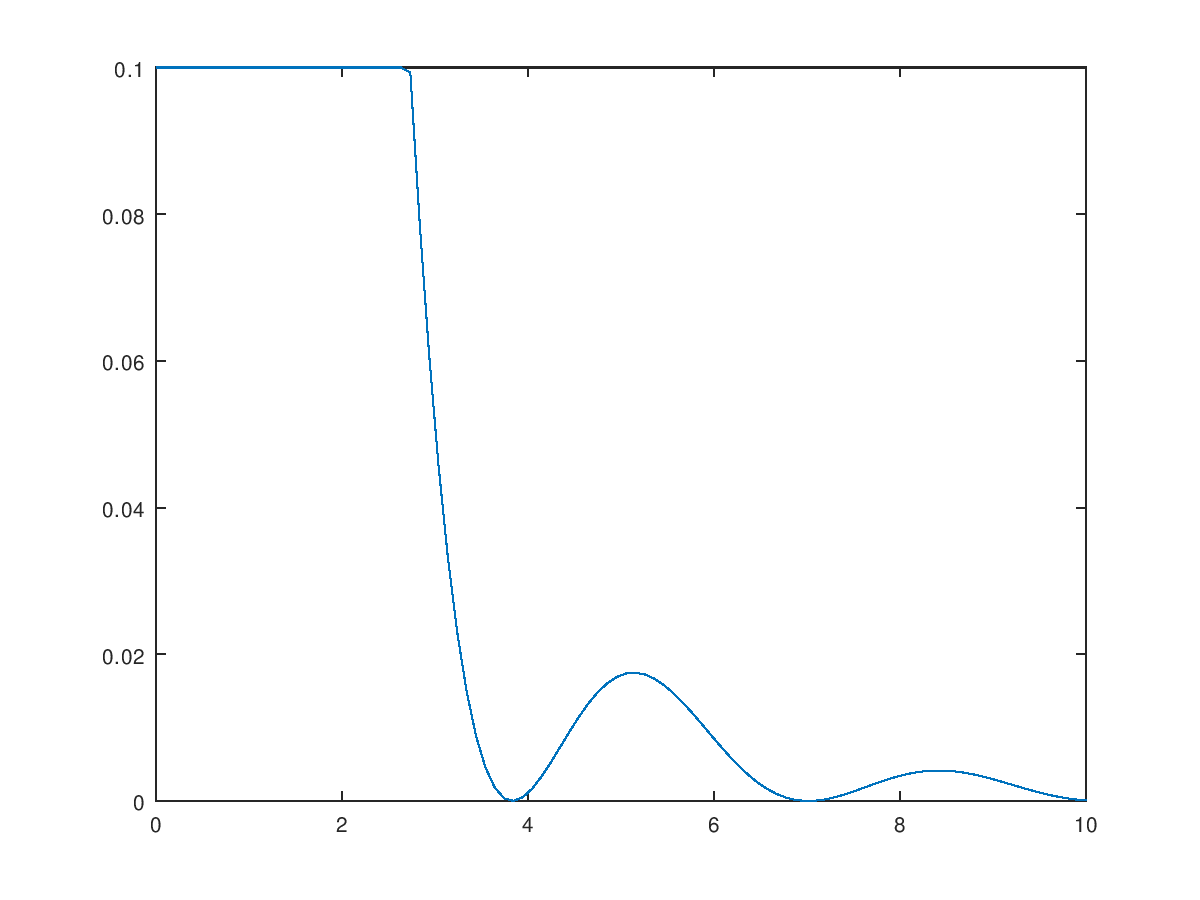
\includegraphics[width=5cm]{profil_1d.png}
\caption{Profil de diffraction tronqué}
\end{figure}

%%%%%%%%%%%%
% Question 2
%%%%%%%%%%%%

2)
\begin{lstlisting}[frame=single]
[x, y] = meshgrid(linspace(-10, 10, 100), linspace(-10, 10, 100));
r = sqrt(x .^ 2 + y .^ 2);
C = 1;
imshow(arrayfun(@(er) k_diffraction(er, C), r));
imshow(arrayfun(@(er) k_diffraction(er, C), r), [0,0.01]);
\end{lstlisting}

\begin{figure}[!h]
\centering
\subfloat[Tache non saturée]{{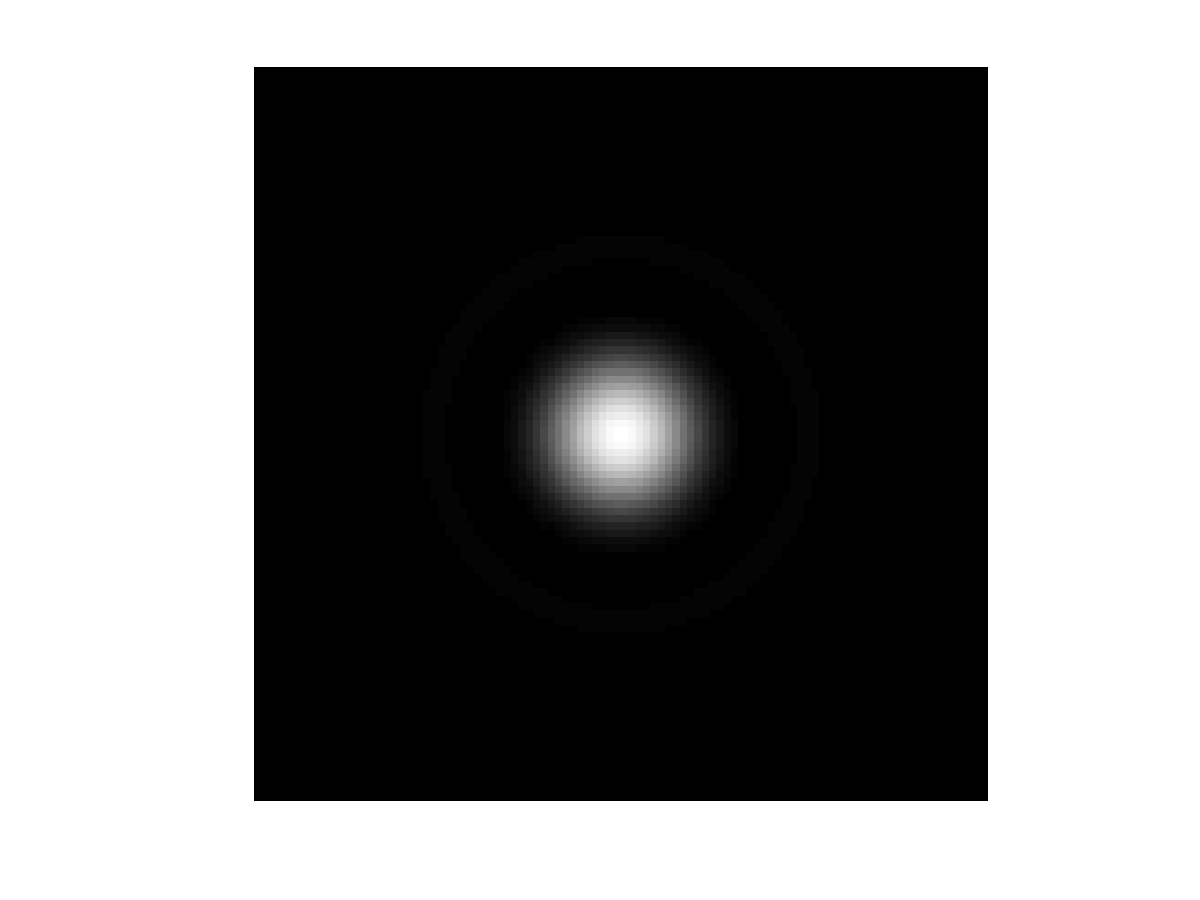
\includegraphics[width=5cm]{airy_no_saturation.png}}}%
\qquad
\subfloat[Tache saturée]{{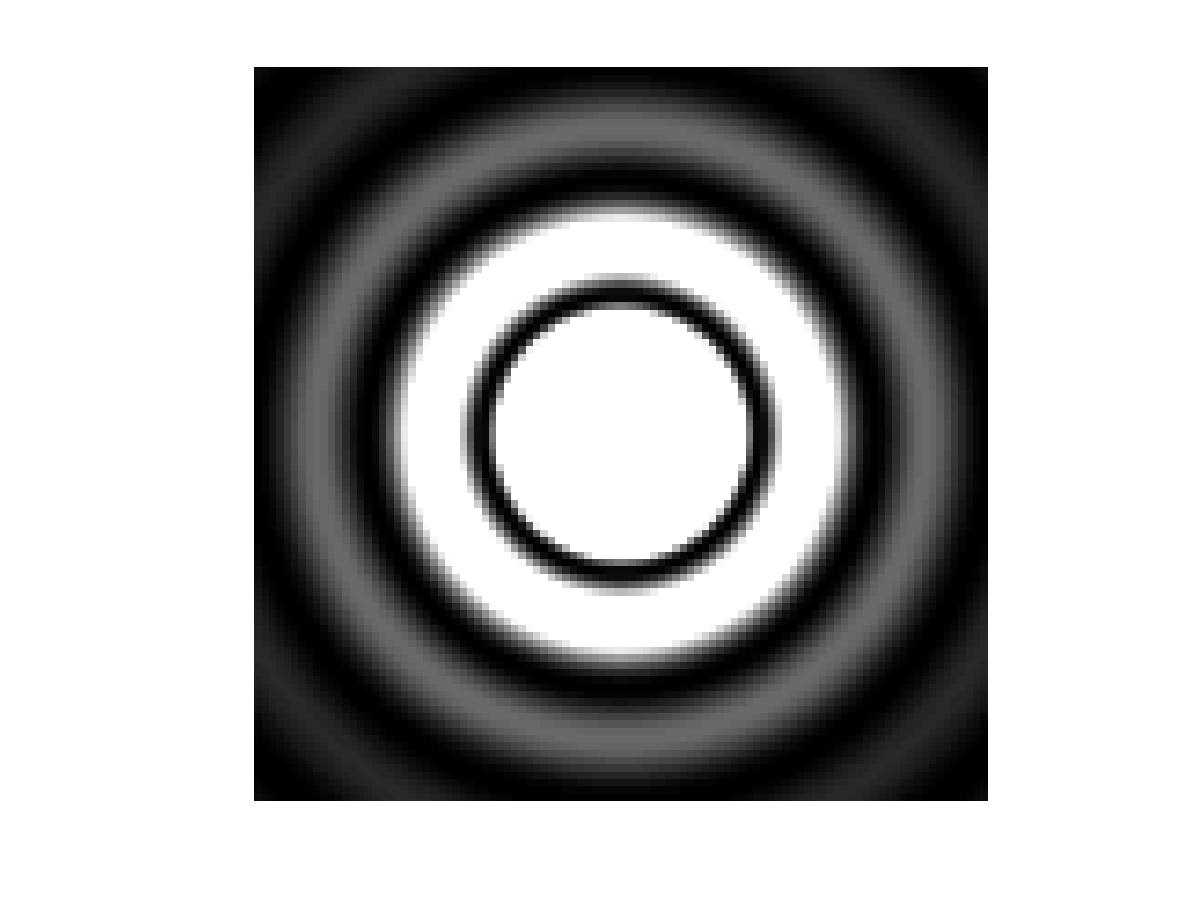
\includegraphics[width=5cm]{airy_avec_saturation.png}}}%
\end{figure}

%%%%%%%%%%%%
% Question 3
%%%%%%%%%%%%

\vbox{
3) On visualise désormais le profil radial et l'image bidimensionnelle de la FTM. 
\begin{lstlisting}[frame=single]
function retval = ftm (x)
    rho=abs(x);
    if (rho >= 1)
        retval = 0;
    else    
        retval=acos(rho)-rho*sqrt(1-rho^2);
endfunction
\end{lstlisting}
}

\begin{lstlisting}[frame=single]
%Profil radial
lr = linspace(0.01, 2, 100);
lf = arrayfun(@(r) ftm(r), lr);
plot(lr,lf);
%Image bidimensionnelle
[x, y] = meshgrid(linspace(-2, 2, 100), linspace(-2, 2, 100));
r = sqrt(x .^ 2 + y .^ 2);
imshow(arrayfun(@(er) ftm(er), r));
\end{lstlisting}


\begin{figure}[!h]
\centering
\subfloat[Profil radial]{{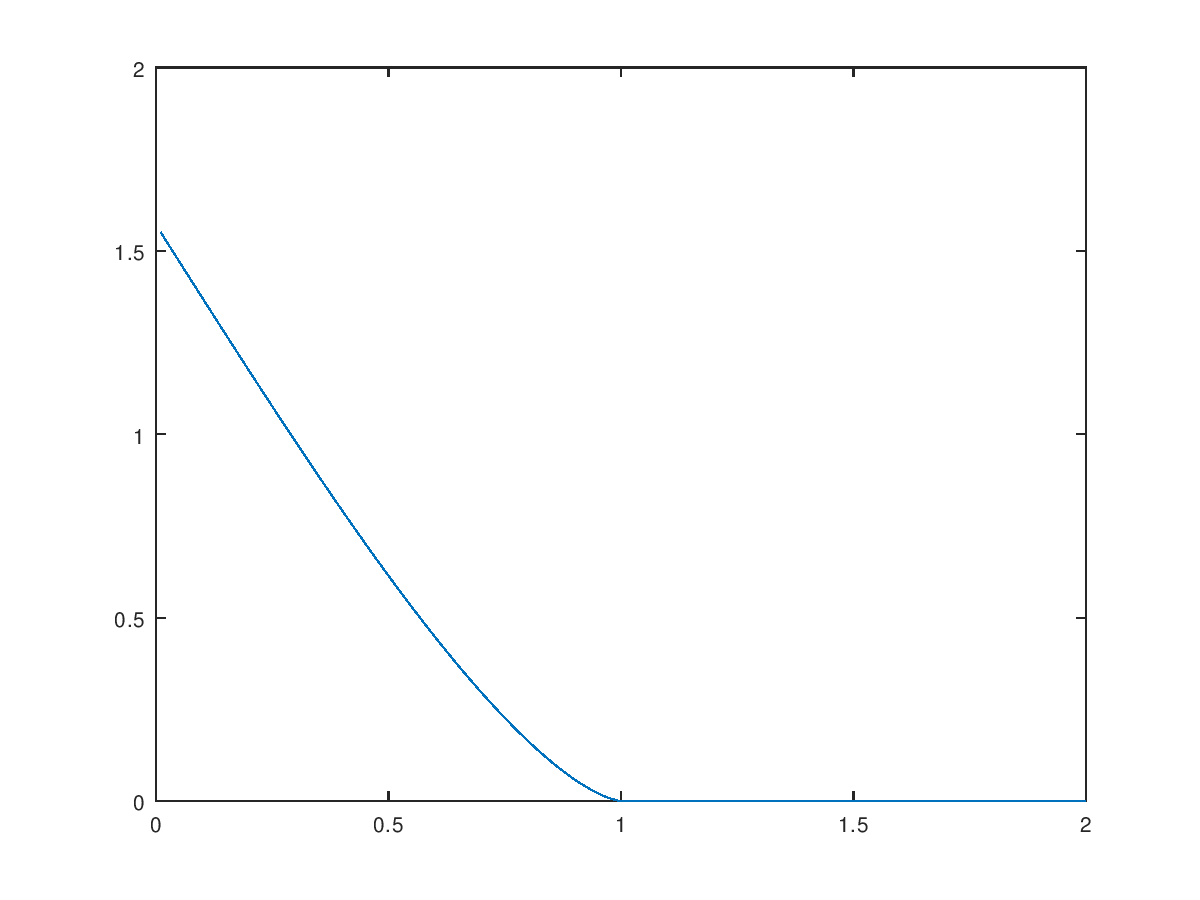
\includegraphics[width=5cm]{ftm_radial.png}}}%
\qquad
\subfloat[Image 2D]{{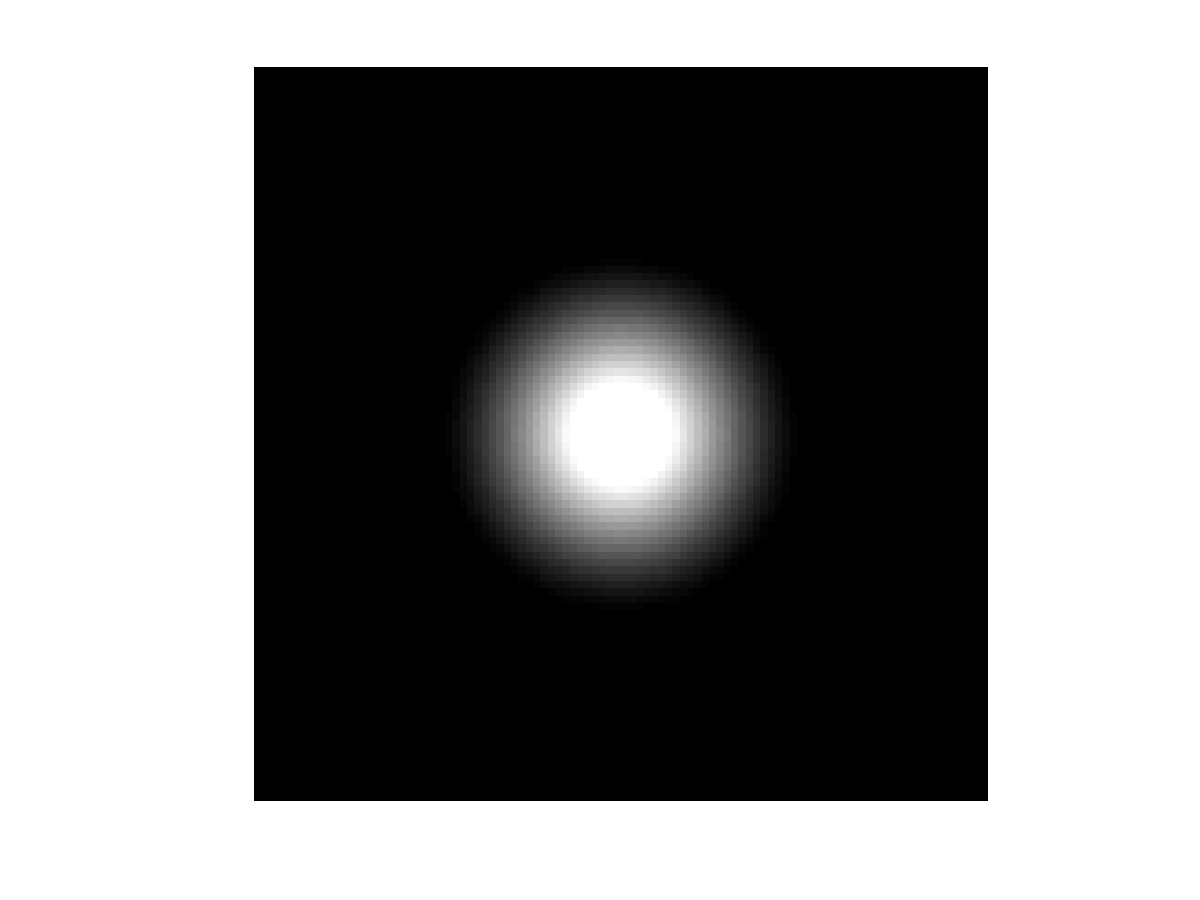
\includegraphics[width=5cm]{ftm_bidim.png}}}%
\end{figure}

\begin{lstlisting}[frame=single]
[x, y] = meshgrid(linspace(-100, 100, 400), linspace(-100, 100, 400));
r = sqrt(x .^ 2 + y .^ 2);
coor = arrayfun(@(er) k_diffraction(er, 1), r);
v = fftshift(abs(fft2(coor)));
imshow(v, [0,max(max(v))]);
\end{lstlisting}

\begin{figure}[!h]
\centering
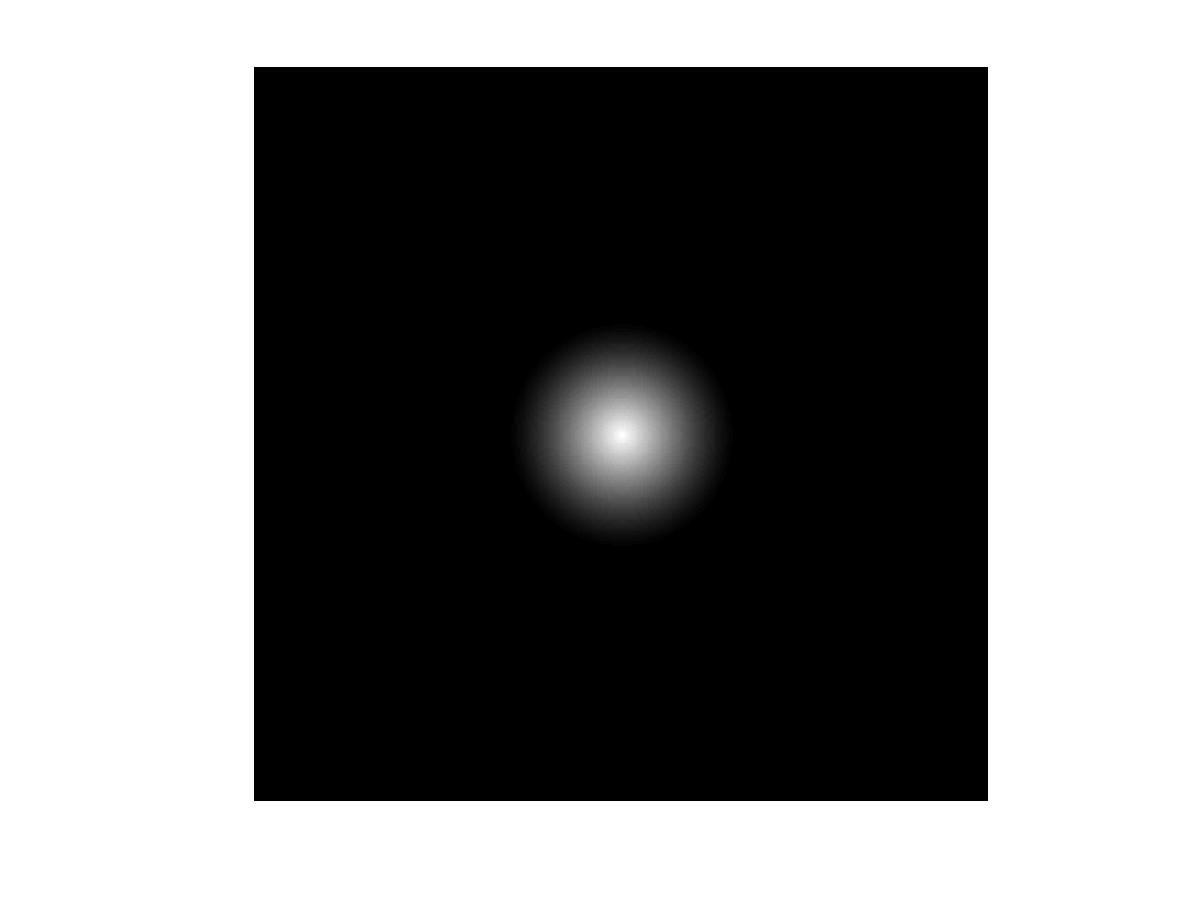
\includegraphics[width=5cm]{ftm_fft2.png}
\caption{FTM calculé par transformée de Fourier discrète à 2D}
\end{figure}

%%%%%%%%%%%%
% Question 4
%%%%%%%%%%%%

4) Comme on peut le voir sur la figure de gauche ci-dessous, les profils superposés présentent deux maxima puis un seul
à mesure que la distance entre les tâches diminue. Etant donné ce graphe, on peut localiser à peu près la distance
critique. On trouve \fbox{critical distance $\approx$ 0.76982$r_a$}.

\begin{figure}[!h]
\centering
\subfloat[Approximate localisation]{{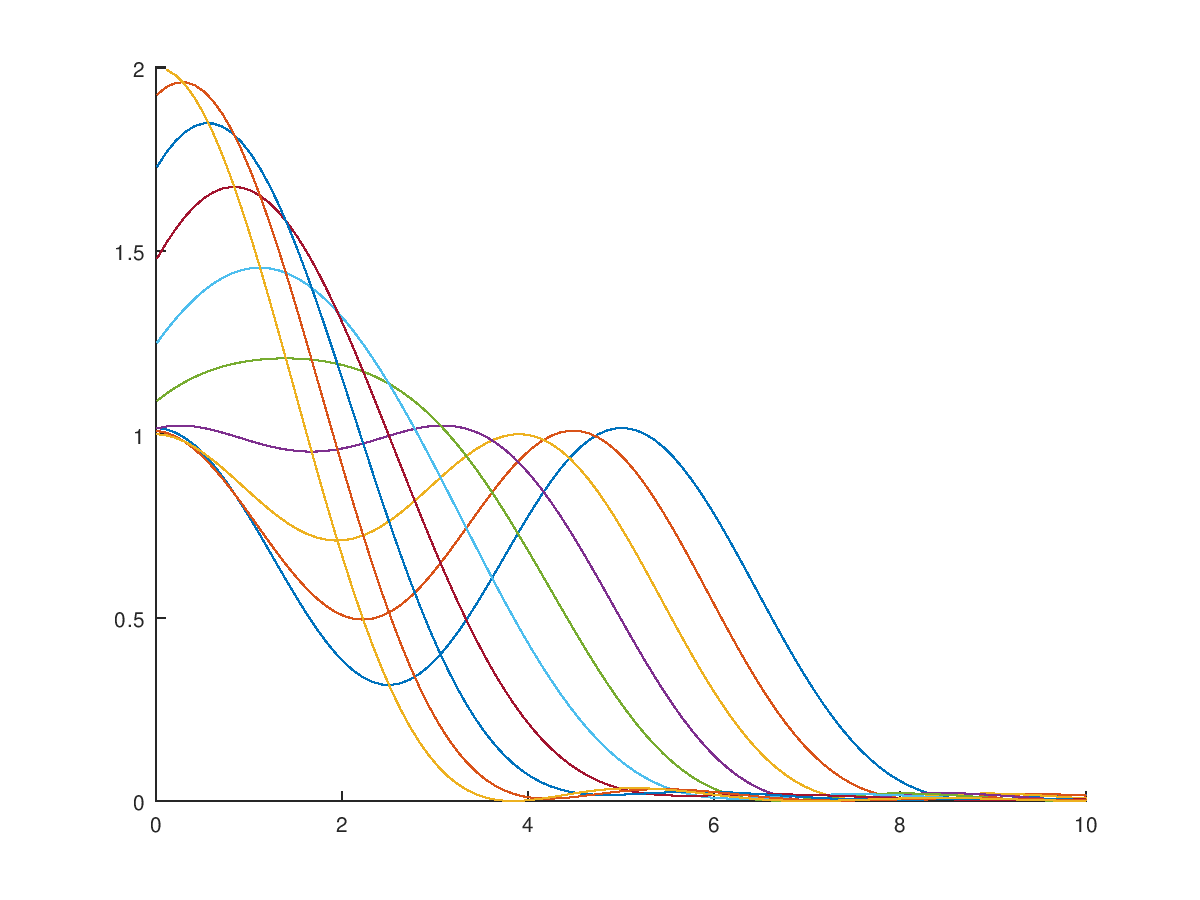
\includegraphics[width=7cm]{approx_dist.png}}}%
\qquad
\subfloat[Exact localisation]{{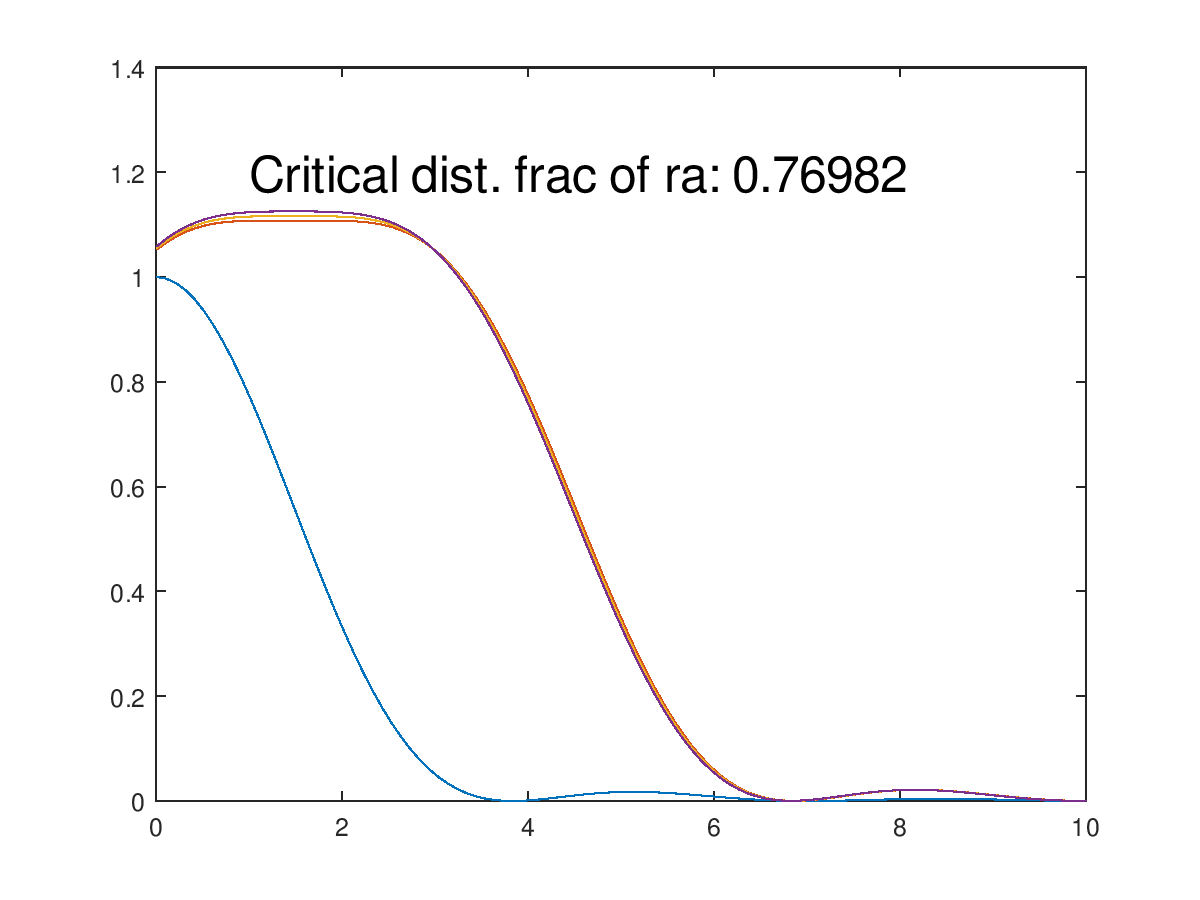
\includegraphics[width=7cm]{exact_dist.png}}}%
\end{figure}

\vbox{\begin{lstlisting}[frame=single]
n_pts = 100;
n_pts_search = 100;
lr = linspace(0.01, 10, n_pts);

% We localised optimal distance in [1,3]
d_search=linspace(3,1, n_pts_search); 
i=0;
n_zeros_x = 4;

% First point spread function
K1 = k_diffraction(lr,1);
[minval, argmin] = min(K1(1:n_pts/2));
ra = lr(argmin);

fprintf("Rayon d'airy:%f\n", ra);
plot(lr, K1)

while n_zeros_x>=2
    i=i+1;
    d=d_search(i);
    rd=abs(lr-d);
    K2=k_diffraction(rd,1);

    % Sum PFS distant from d
    K=K1+K2;
    diff_K = diff(K);
    
    % Count number of zero crossings in the range 0 to d
    % If this is higher than 1, there are at least 2 extrema
    
    [minval, argmin] = min(abs(lr-d));
    f_idx = 1;
    l_idx = argmin-1;
    n_zeros_x = count_zeros(diff_K(f_idx:l_idx));
    hold on
    plot(lr,K)
end
fprintf("Critical distance as fraction of ra: %f\n", d/ra)
\end{lstlisting}}

%%%%%%%%%%%%
% Question 5
%%%%%%%%%%%%

\vbox{5) En reprenant les calculs vus en cours on a pour une pupille s'étandant sur le domaine $\{x | \epsilon \frac{D}{2} \leq
\left\Vert{x}\right\Vert \leq \frac{D}{2}\}$

\begin{align*}
K_{diffraction}(x) & = \frac{1}{2f^2} \left| \int_{\epsilon \frac{D}{2}}^{\frac{D}{2}} 2\pi J_0(\frac{2\pi|x|r}{\lambda
f}) r dr \right| ^2 \\
& = \frac{\pi^2 D^4}{8f^2 R^4} \big(R J_1(R) - (\epsilon R) J_1(\epsilon R)\big)^2 \\ 
& = C \Big(\frac{2 J_1(R)}{R}\Big)^2 + C \Big(\frac{2 \epsilon J_1(\epsilon R)}{R}\Big)^2 - 8C\frac{J_1(R)\epsilon
J_1(\epsilon R)}{R^2}
\end{align*}}

%%%%%%%%%%%%
% Question 6
%%%%%%%%%%%%

6) On définit une fonction pour calculer le noyau de diffraction associé à une pupille de télescope.
\begin{lstlisting}[frame=single]
function [y] = k_diffraction_telesc (r, C, ep)
    jr = besselj(1, r);
    jr_ep = besselj(1,ep .* r);
    y = C * (2 .* jr ./ r) .** 2 -  C * (2 * ep .* jr_ep ./ r) .** 2 - 8*C*(ep.* jr .* jr_ep) ./ r^2; 
endfunction
\end{lstlisting}

On réexecute la transformation de Fourier discrète avec cette nouvelle fonction pour visualiser la FTM.

\begin{lstlisting}[frame=single]
[x, y] = meshgrid(linspace(-100, 100, 400), linspace(-100, 100, 400));
r = sqrt(x .^ 2 + y .^ 2);
coor = arrayfun(@(er) k_diffraction_telesc(er, 1, 1/4), r);
v = fftshift(abs(fft2(coor)));
imshow(v, [0,max(max(v))]);
\end{lstlisting}

\begin{figure}[!h]
\centering
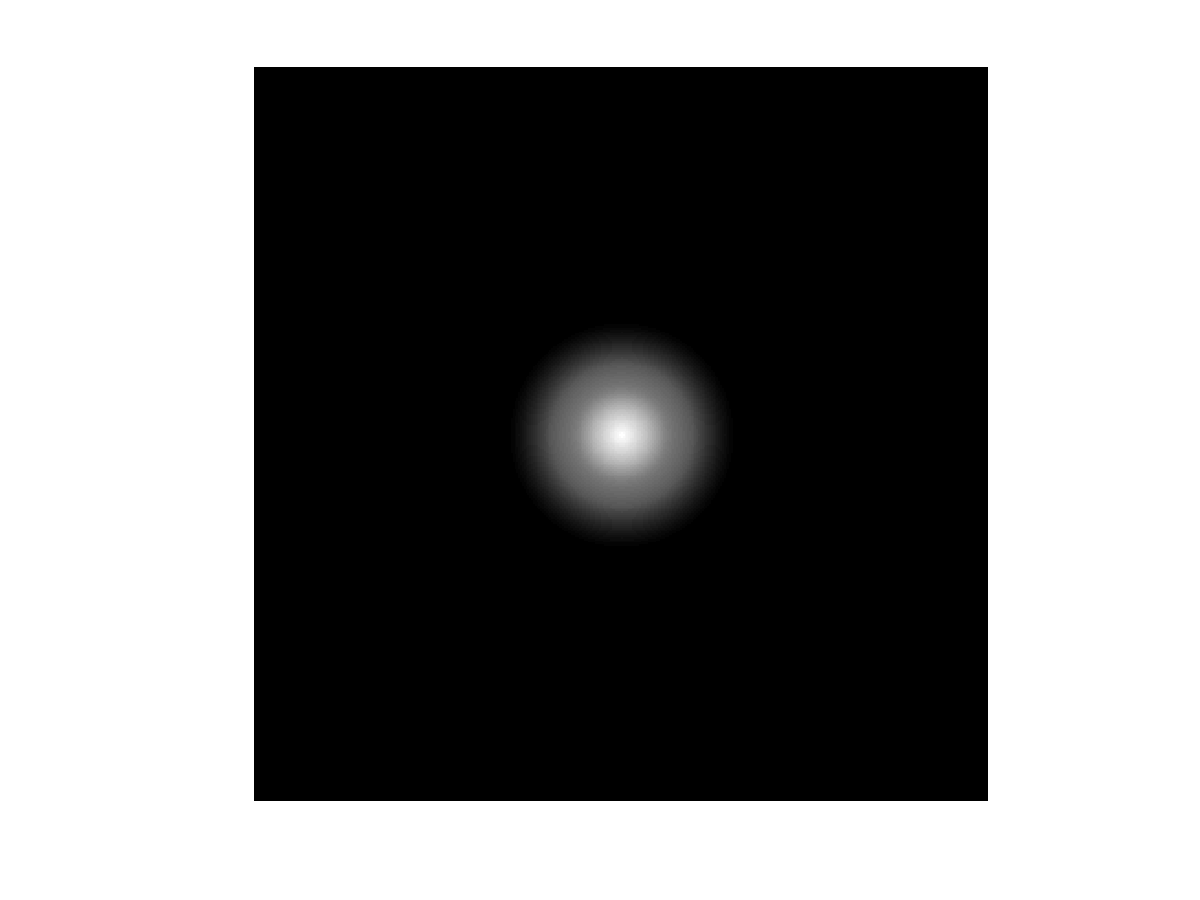
\includegraphics[width=5cm]{ftm_telesc_fft2.png}
\caption{FTM télescope calculée par transformée de Fourier discrète à 2D}
\end{figure}

On observe la même FTM que pour une pupille de même diamètre sans occlusion. On en déduit que la lunette et le télescope
ont la même résolution. 

\paragraph{Exercice 2}

%%%%%%%%%%%%
% Question 1
%%%%%%%%%%%%

1) $g$ étant mesurable à support compact, elle est dans $L^1(\mathbf{R}^2)$. Définissons $\tilde{g}$ la fonction
$\tilde{g} : x \to g(-x)$. Alors $\tilde{g}$ est aussi dans $L^1$ et:

\begin{align*}
\Gamma & = \tilde{g} \star g \\
\text{d'où} \quad \hat{\Gamma}(\xi) & = \widehat{\tilde{g} \star g}(\xi) \\ 
& = \hat{\tilde{g}}(\xi) \times \hat{g}(\xi) \\
& = \int_{\mathbf{R}^2} g(x) e^{+i<x,\xi>} dx \times \int_{\mathbf{R}^2} g(x) e^{-i<x,\xi>} dx \\
& = \left|\hat{g}(\xi)\right|^2
\end{align*}

En effet, dans l'avant dernière ligne les intégrales sont conjuguées l'une de l'autre et la seconde est la transformée
de Fourier de g.

\end{document}

